\documentclass{acm_proc_article-sp}

\usepackage{graphicx}% Include figure files
\usepackage{dcolumn}% Align table columns on decimal point
\usepackage{bm}% bold math
\usepackage{float}
\usepackage{array}
\usepackage{verbatim}
\usepackage{hyperref}% add hypertext capabilities
%\usepackage[mathlines]{lineno}% Enable numbering of text and display math
%\linenumbers\relax % Commence numbering lines

\usepackage{listings}
\usepackage{footnote}
\makesavenoteenv{table}
\makesavenoteenv{table*}
\makesavenoteenv{tabular}

\begin{document}

\title{Self organizing systems WS14 - Exercise 2\\
       Self Organizing Maps}% Force line breaks with \\

\numberofauthors{2}
\author{
\alignauthor
Dragan Avramovski\\
       \email{e1426093@student.tuwien.ac.at}
\alignauthor
Richard Plangger\\
 \email{e1025637@student.tuwien.ac.at}
}

\date{\today}

\maketitle


\begin{abstract}
\end{abstract}

\keywords{Self organizing systems, SOM }

\section{Wine dataset}

For our dataset we chose the ``wine-quality'' dataset from the UCI Machine Learning Repository~\cite{ucirepo}. 
Herefater the dataset is called WQ.
It is data from wine variants of a Portoguese wine called ``Vino Verde''.
The data points the quality measure are physicochemical values measured
by sensors or tests. There is no information about the grape types,
wine brand, selling prices of the wine.
WQ has 12 different attributes and more than 6500 instances of red and white wine listed in the following enumeration:

\begin{itemize}
    \item Fixed acidity
    \item Volatile acidity
    \item Citric acid
    \item Residual sugar
    \item Chlorides
    \item Free sulfur dioxide
    \item Total sulfur dioxide
    \item Density
    \item pH
    \item Sulphates
    \item Alcohol
    \item Quality (A score between 0 and 10)
\end{itemize}

The data set contains two seperate data files. One for white wine,
another for red wine. We merged the two together into a monolitic file,
and appending the wine type as a new attribute. $1$ denotes red wine, $2$ white wine.

The attribute quality is the only attribute that are human decided.
Each data entry has at least opinions of three different experts. This
sensory data is collected and the median the value included in the
dataset.

\section{Normalisation and data cleaning}

To get a feeling of the distribution of the data we used
WEKA to plot each attribute along its value range to visualise
density and the distribution.
Figure~\ref{fig:dist-alcohol} shows the distribution of the alcohol attribute. pH has
also a very similar distribution and both do not seem to have outliers.
For these two attributes we apply min max scaling.

\begin{figure}
\centering
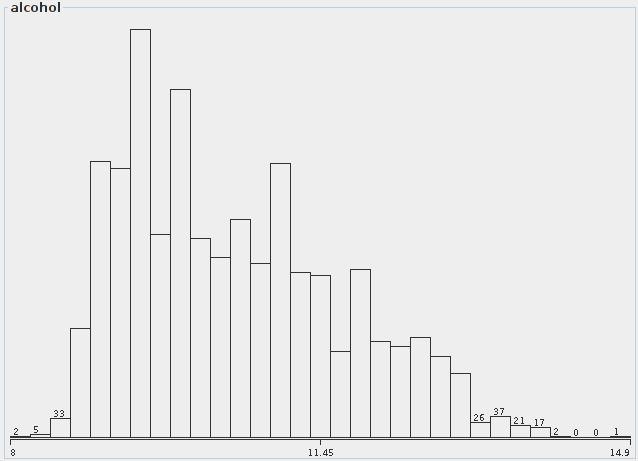
\includegraphics[width=\linewidth]{img/dist-alcohol}
\caption{Data distribution of the alcohol attribute (not normalized)}
\label{fig:dist-alcohol}
\end{figure}

\begin{comment}
    \begin{figure}
    \centering
    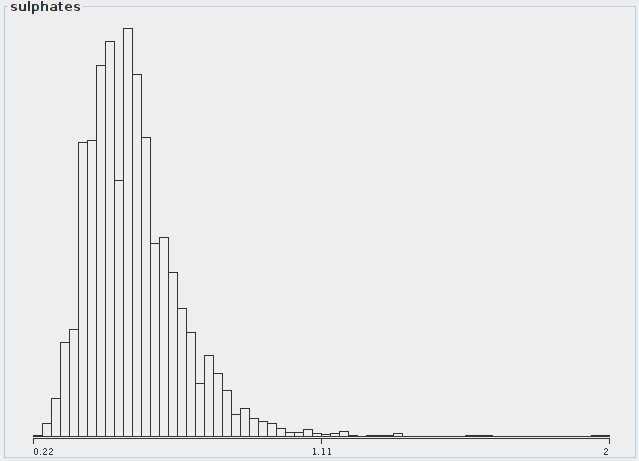
\includegraphics[width=\linewidth]{img/dist-sulphates}
    \caption{Data distribution of the sulphate attribute (not normalized)}
    \label{fig:dist-sulphates}
    \end{figure}
\end{comment}


For Fixed/Volatile acidity and Total sulfur dioxide we apply Zero Mean Variance scaling. For these three we 
believe that the few outliers are features, not noise in the measurements.
For all others\footnote{Citri acid, Residual Sugar, Chlorides, Free/Total sulfur dioxide, Density, Sulphates}
we decided to exclude data samples with the outliers. The Table~\ref{tab:cutoff} shows the threshold after we drop
the data record. In Figure~\ref{fig:dist-citric-acid} a sample of the not normalized data is shown. A lot
of samples have a value to the left of the attribute range. Figure~\ref{fig:ndist-citric-acid} shows the
normalized attribute range.

\begin{figure}
\centering
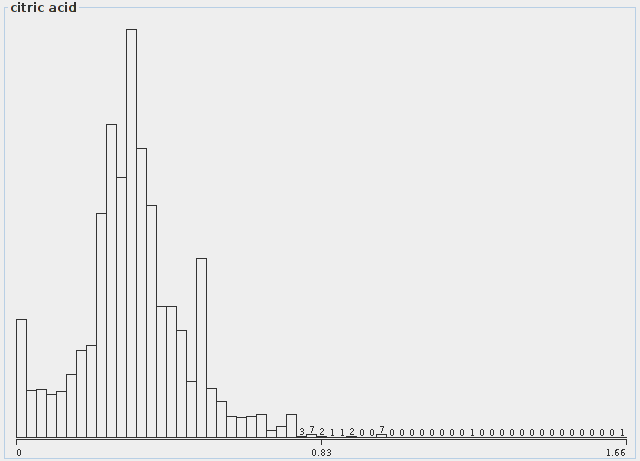
\includegraphics[width=\linewidth]{img/dist-citric-acid}
\caption{Data distribution of the citric acid attribute (not normalized)}
\label{fig:dist-citric-acid}
\end{figure}

\begin{figure}
\centering
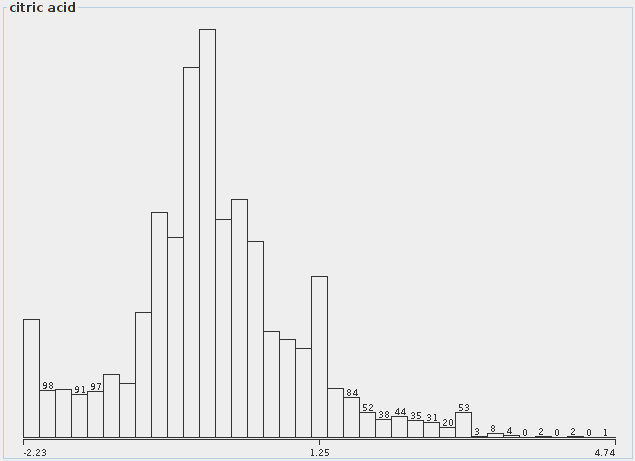
\includegraphics[width=\linewidth]{img/ndist-citric-acid}
\caption{Data distribution of the citric acid attribute (normalized)}
\label{fig:ndist-citric-acid}
\end{figure}

\begin{table}
\centering
\begin{tabular}{l|c}
    Attribute & Cutoff \\
    \hline
    \hline
    Citri acid & 1.0 \\
    \hline
    Residual Sugar & 30.0 \\
    \hline
    Chlorides & 0.3 \\
    \hline
    Free sulfur dioxide & 150 \\
    \hline
    Density & 1.01 \\
    \hline
    Sulphates & 1.3 \\
\end{tabular}
\caption{Table that shows the cutoff for normalizations}
\label{tab:cutoff}
\end{table}

The total amount of rows that are filtered are 44 rows. This decreases the data set from 6497 instances to 6453.
We provide the original data samples in a file called ``wq.csv'', the samples that do not include quality and type
in ``wq-n-o.csv'' and the normalized data in ``wq-n.csv''.

We also decided to subsample the dataset and only include 3000 random samples. In our
automated script we used Python 2.7 and subsampled using a random seed of 0.


\section{Training the first SOM}

\[ \alpha = 0.7,
   \sigma = 7,
   s_x = 14,
   s_y=10,
   i=500,
   r = 7, 
\]

\bibliography{ref}
\bibliographystyle{plain}



\end{document}
